\subsection{Regression mit ARMA-Fehlern}
\begin{frame}{Autokorrelation der Datenübertragungsrate (Uplink)}
	\begin{figure}
		%\centering
		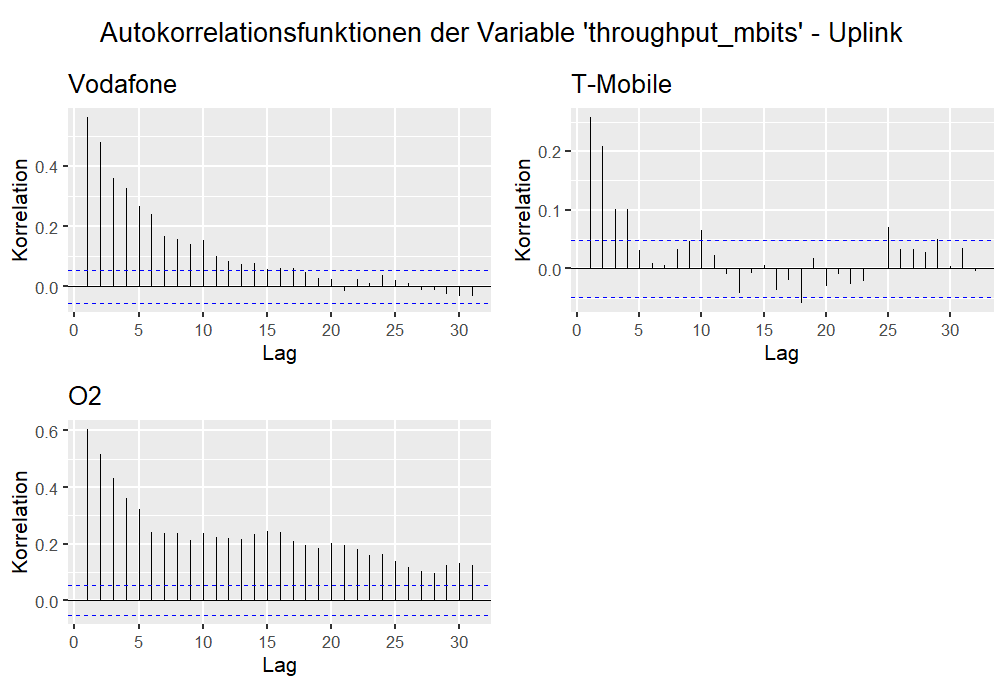
\includegraphics[scale=0.38]{plots/arima/uplink/throughput_acf}\\
		\caption{Autokorrelationsfunktion der Datenübertragungsrate in Richtung Uplink.}
		\label{throughput_acf}
	\end{figure}
\end{frame}

\begin{frame}{partielle Autokorrelation der Datenübertragungsrate(Uplink)}
	\begin{figure}
		%\centering
		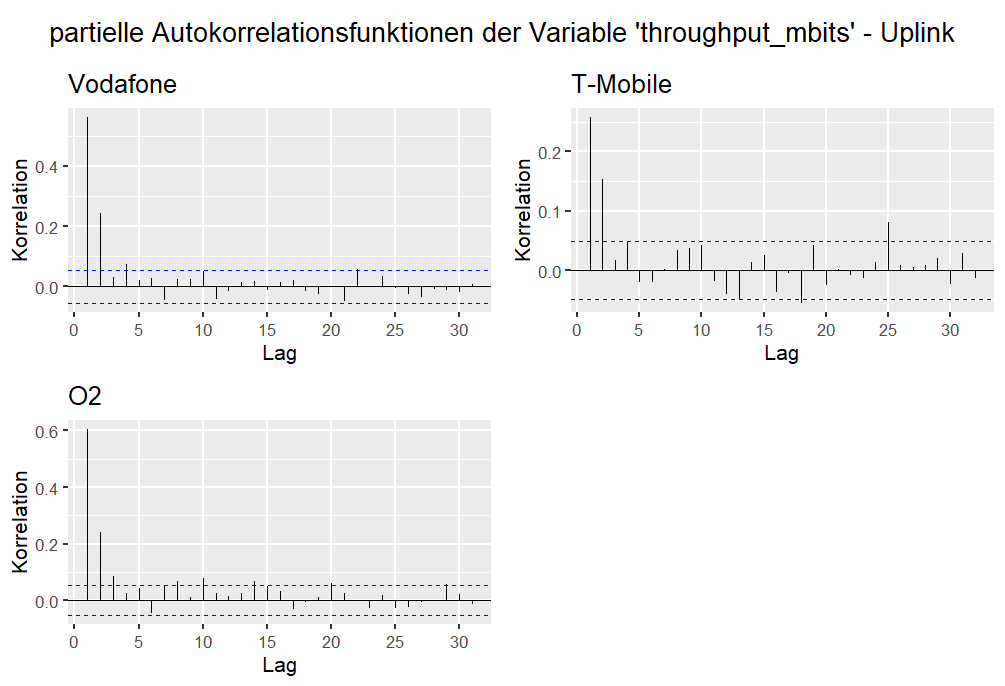
\includegraphics[scale=0.38]{plots/arima/uplink/throughput_pacf}\\
		\caption{partielle Autokorrelationsfunktion der Datenübertragungsrate in Richtung Uplink.}
		\label{throughput_pacf}
	\end{figure}
\end{frame}

\begin{frame}{Test auf Stationarität (Uplink)}
	\textbf{Augmented Dickey-Fuller Test} \cite{time_series_analysis}:\\
	H$_0$: Zeitreihe hat Einheitswurzel $\Rightarrow$ Zeitreihe ist nicht stationär\\
	H$_1$: Zeitreihe hat keine Einheitswurzel $\Rightarrow$ Zeitreihe ist stationär
	\begin{figure}
		\begin{tabular}{l||c|c|c}
			\textbf{Feature} & \textbf{Vodafone} & \textbf{T-Mobile} & \textbf{O2} \\
			\hline\hline
			\textbf{throughput\_mbits} & 0,01 & 0,01 & 0,01 \\
			\textbf{payload\_mb} & 0,01 & 0,01 & 0,01 \\
			\textbf{f\_mhz} & 0,01 & 0,045 & 0,01 \\
			\textbf{rsrp\_dbm} & 0,01 & 0,01 & 0,01 \\
			\textbf{rsrq\_db} & 0,01 & 0,01 & 0,01 \\
			\textbf{rssnr\_db} & 0,01 & 0,01 & 0,01 \\
			\textbf{cqi} & 0,01 & 0,01 & 0,01 \\
			\textbf{ta} & 0,01 & 0,01 & 0,01 \\
			\textbf{velocity\_mps} & 0,01 & 0,01 & 0,01 \\
			\textbf{enodeb} & 0,01 & 0,01 & 0,01 \\
		\end{tabular}
		\caption{Ergebnisse des Augmented Dickey-Fuller Tests auf Stationarität für alle Variablen in Richtung Uplink.}
	\end{figure}
\end{frame}

\begin{frame}{Überprüfung der Multikollinearität (Uplink)}
	\textbf{Varianzinflationsfaktor (VIF)} \cite{fahrmeir_regression}:\\
	$\text{VIF}=\frac{1}{1-R^2_j}$ gibt an, um welchen Faktor die Varianz von $\beta_j$ durch lineare Abhängigkeit vergrößert wird. \underline{Faustregel}: VIF $<10$
	\begin{figure}
		\begin{table}
			%\centering
			%\resizebox{7cm}{2.4cm}{%
			\begin{tabular}{l||c|c|c}
				\textbf{Feature} & \textbf{Vodafone} & \textbf{T-Mobile} & \textbf{O2} \\
				\hline\hline
				\textbf{payload\_mb} & 1,01 & 1,00 & 1,00 \\
				\textbf{f\_mhz} & 1,45 & 1,26 & 1,50 \\
				\textbf{rsrp\_dbm} & 2,65 & 2,02 & 1,81 \\
				\textbf{rsrq\_db} & 2,39 & 2,21 & 2,81 \\
				\textbf{rssnr\_db} & 2,78 & 2,62 & 3,44 \\
				\textbf{cqi} & 2,05 & 1,84 & 2,71 \\
				\textbf{ta} & 1,38 & 1,27 & 1,23 \\
				\textbf{velocity\_mps} & 1,13 & 1,27 & 1,21 \\
				\textbf{enodeb} & 1,20 & 1,29 & 1,05 \\
			\end{tabular}%
			%}
		\end{table}
		\caption{Varianzinflationsfaktor aller Einflussvariablen in Richtung Uplink.}
	\end{figure}
\end{frame}

\begin{frame}{Normalverteilung der Residuen (Uplink)}
	\begin{figure}
		%\centering
		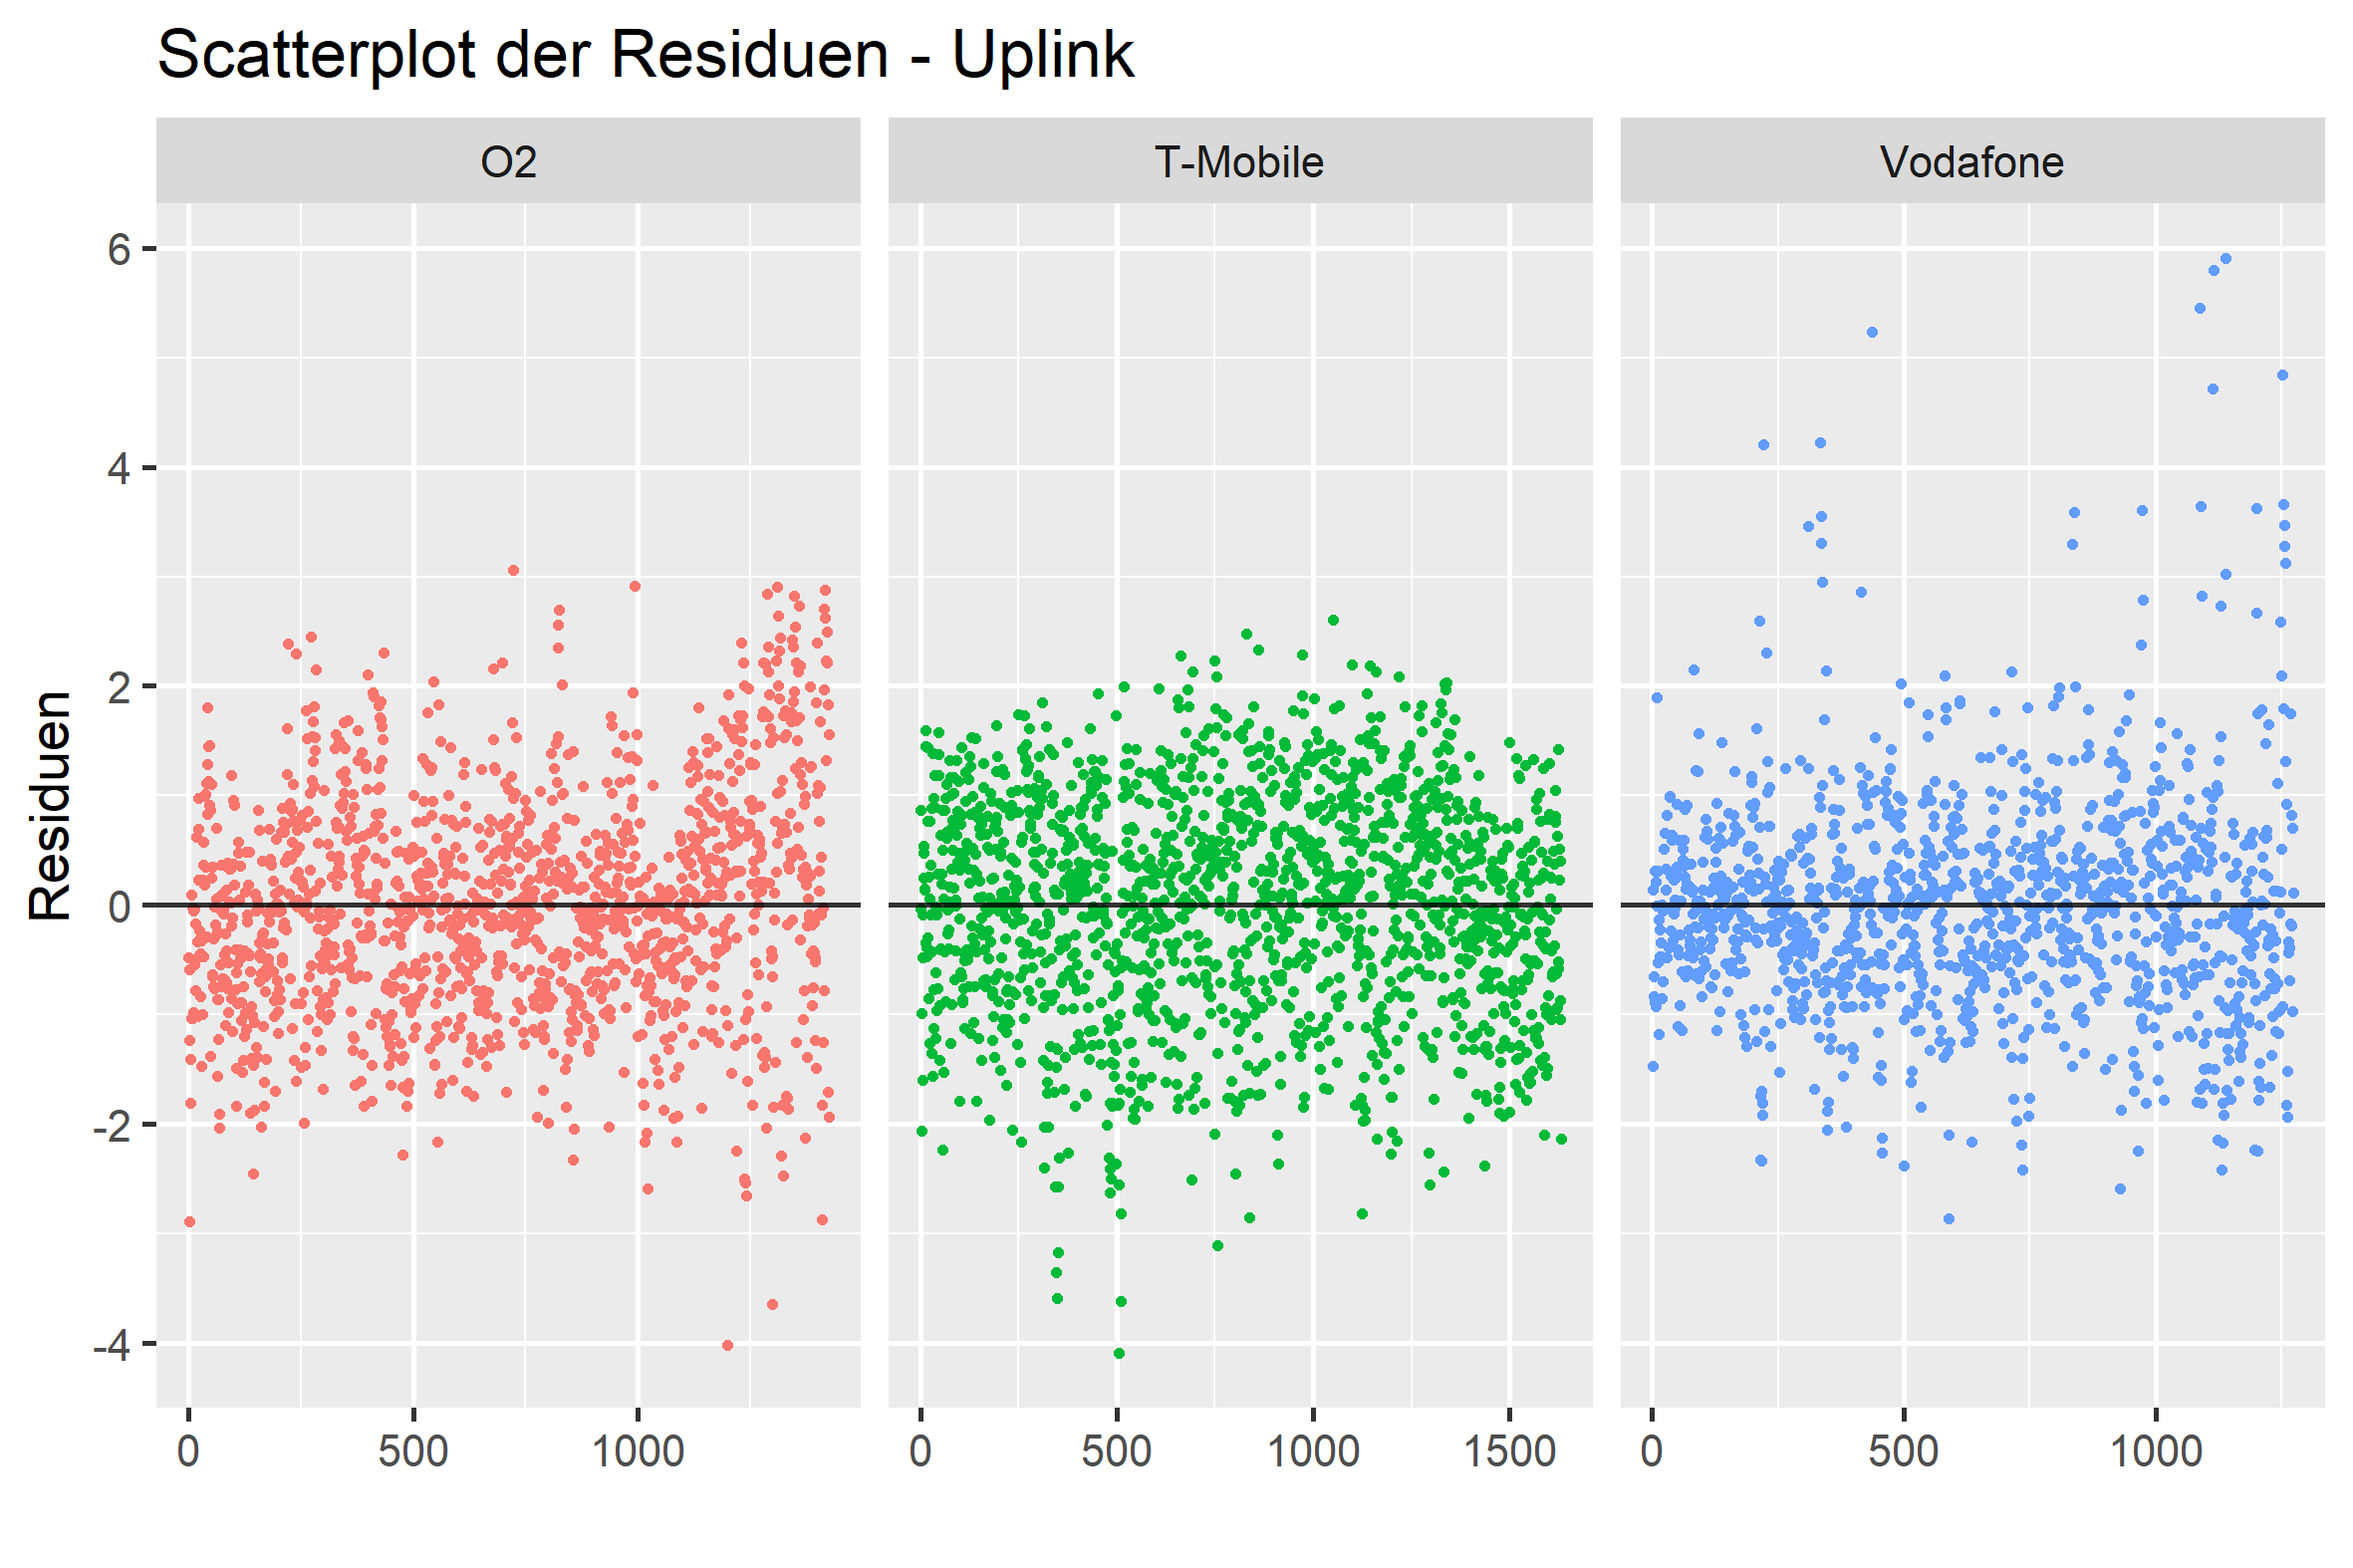
\includegraphics[scale=0.35]{plots/arima/uplink/res_scatter}\\
		\caption{Scatterplots der Residuen der linearen Modelle mit Daten der Richtung Uplink.}
		\label{res_scatter}
	\end{figure}
\end{frame}
\begin{frame}{Normalverteilung der Residuen (Uplink)}
	\begin{figure}
		%\centering
		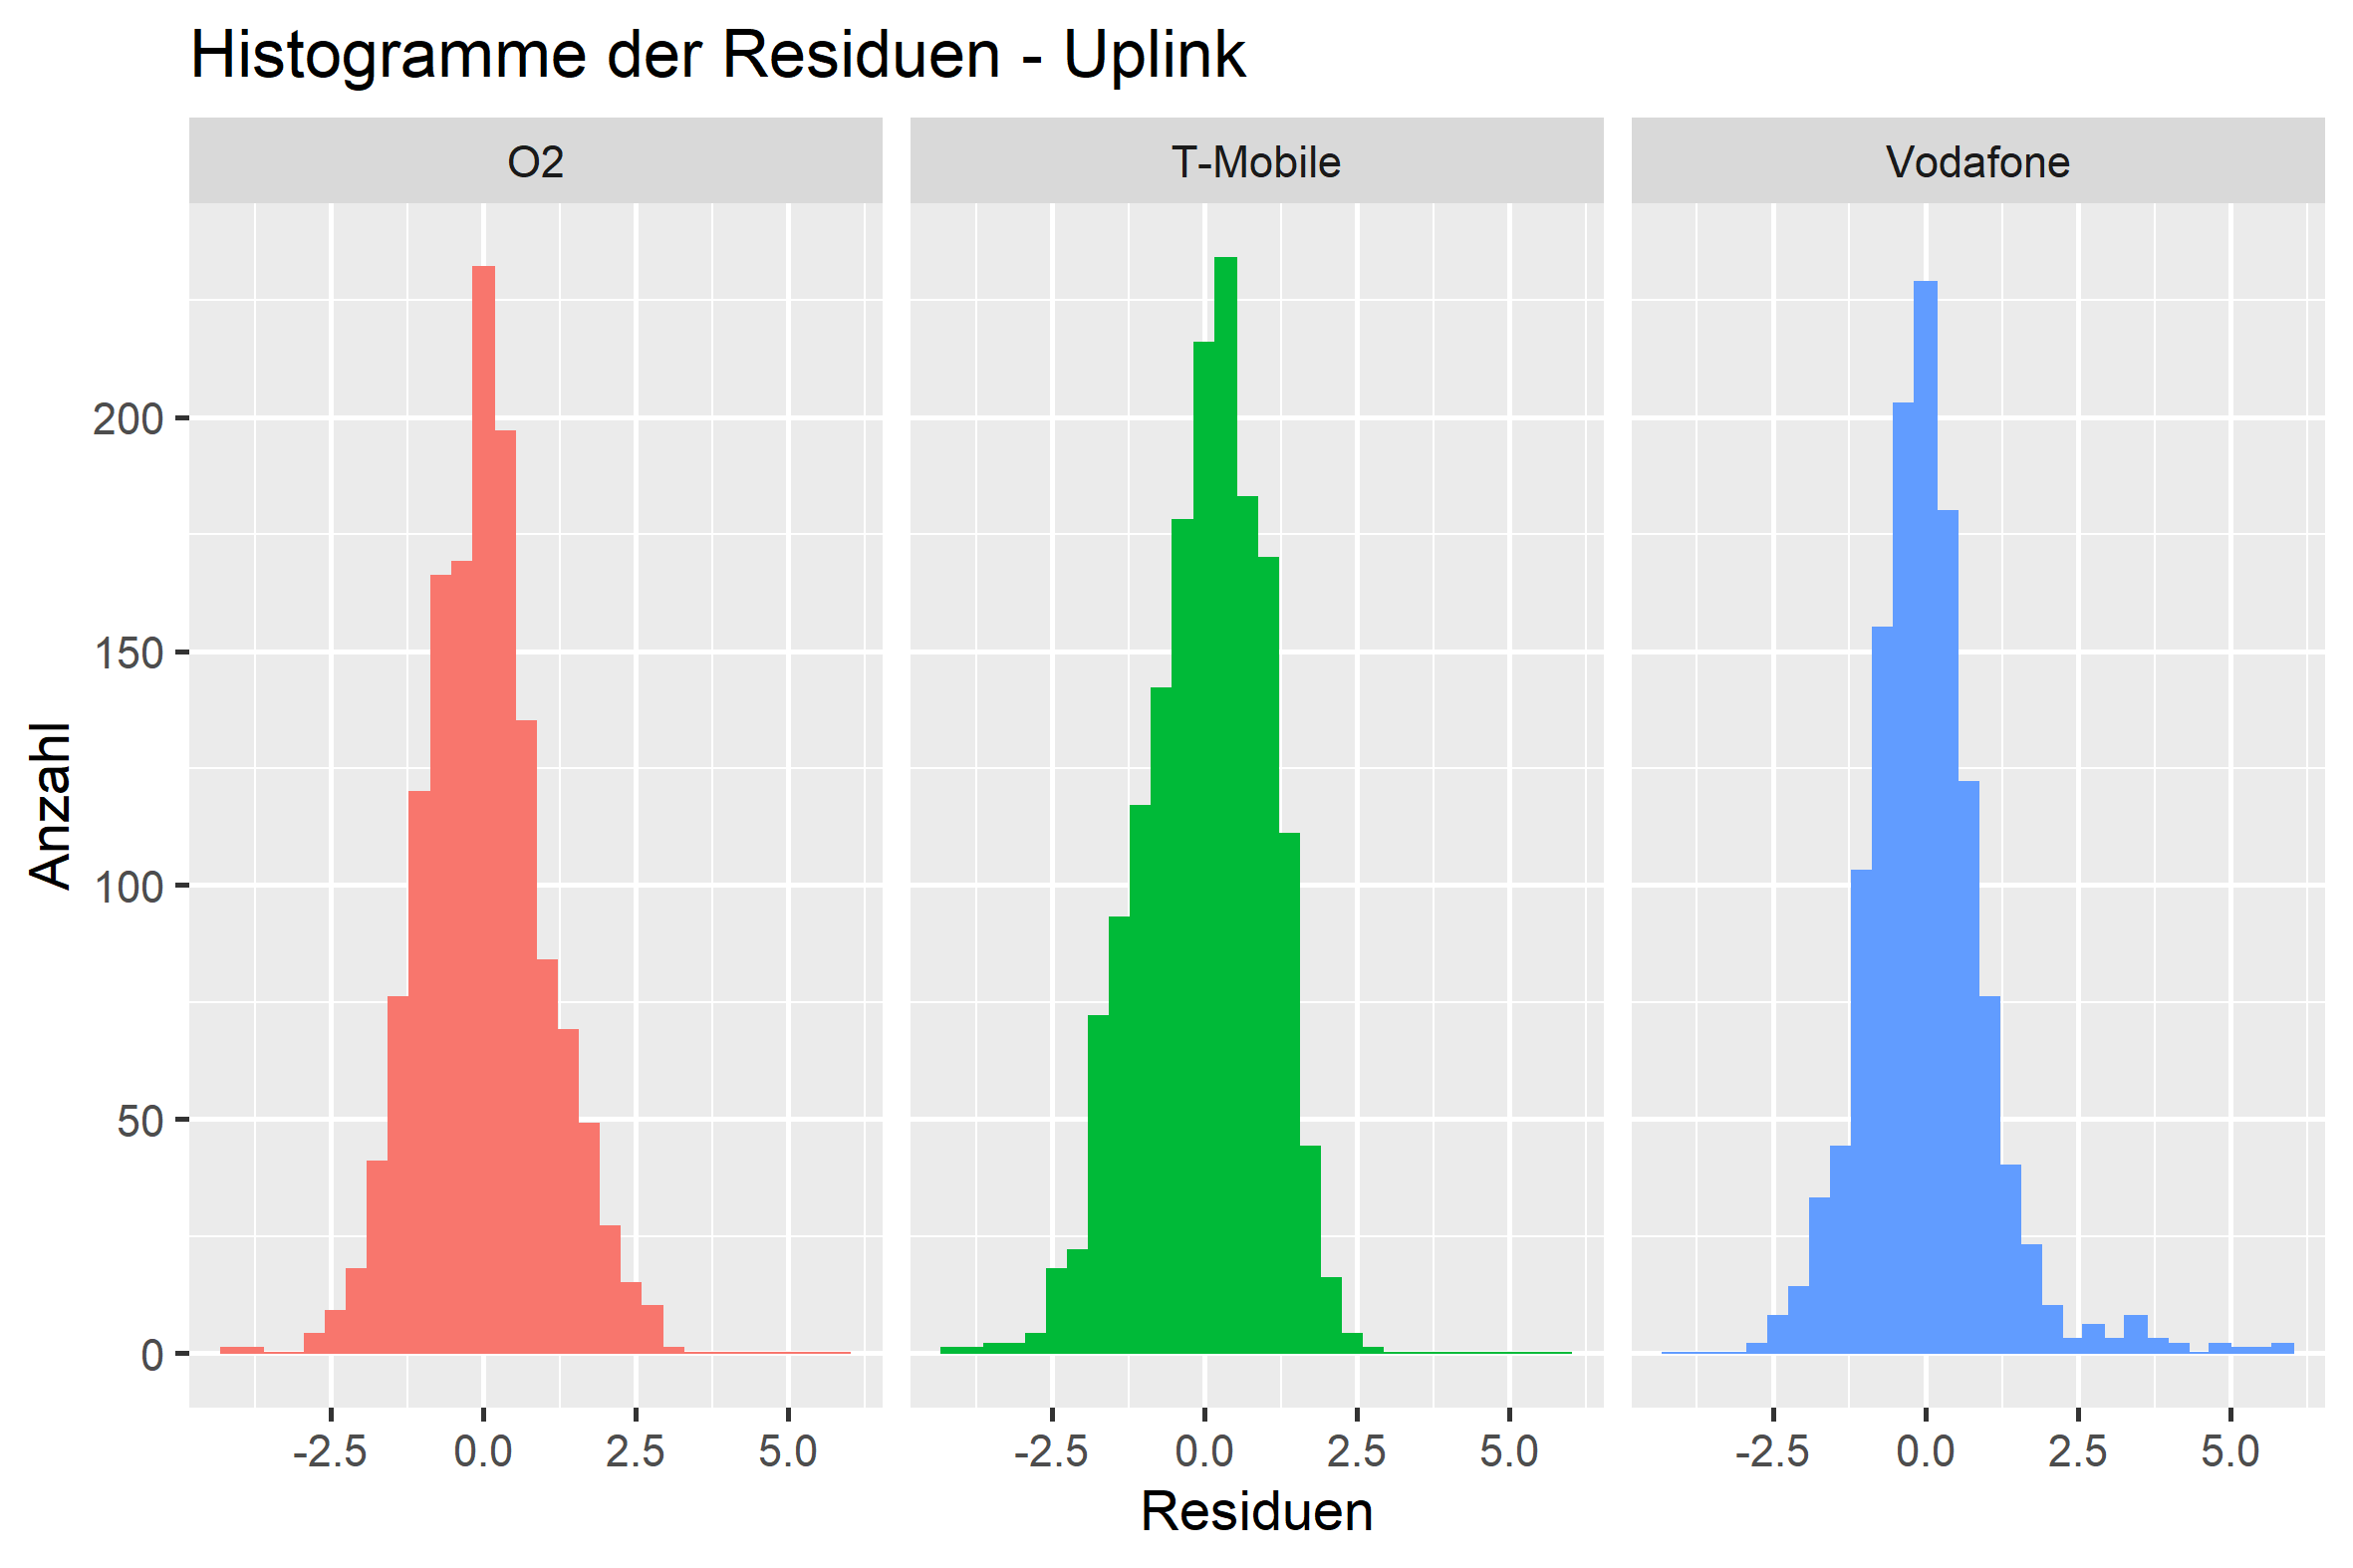
\includegraphics[scale=0.35]{plots/arima/uplink/res_histogram}\\
		\caption{Histogramme der Residuen der linearen Modelle mit Daten der Richtung Uplink.}
		\label{res_histogram}
	\end{figure}
\end{frame}

\begin{frame}{Normalverteilung der Residuen (Uplink)}
	\begin{figure}
		%\centering
		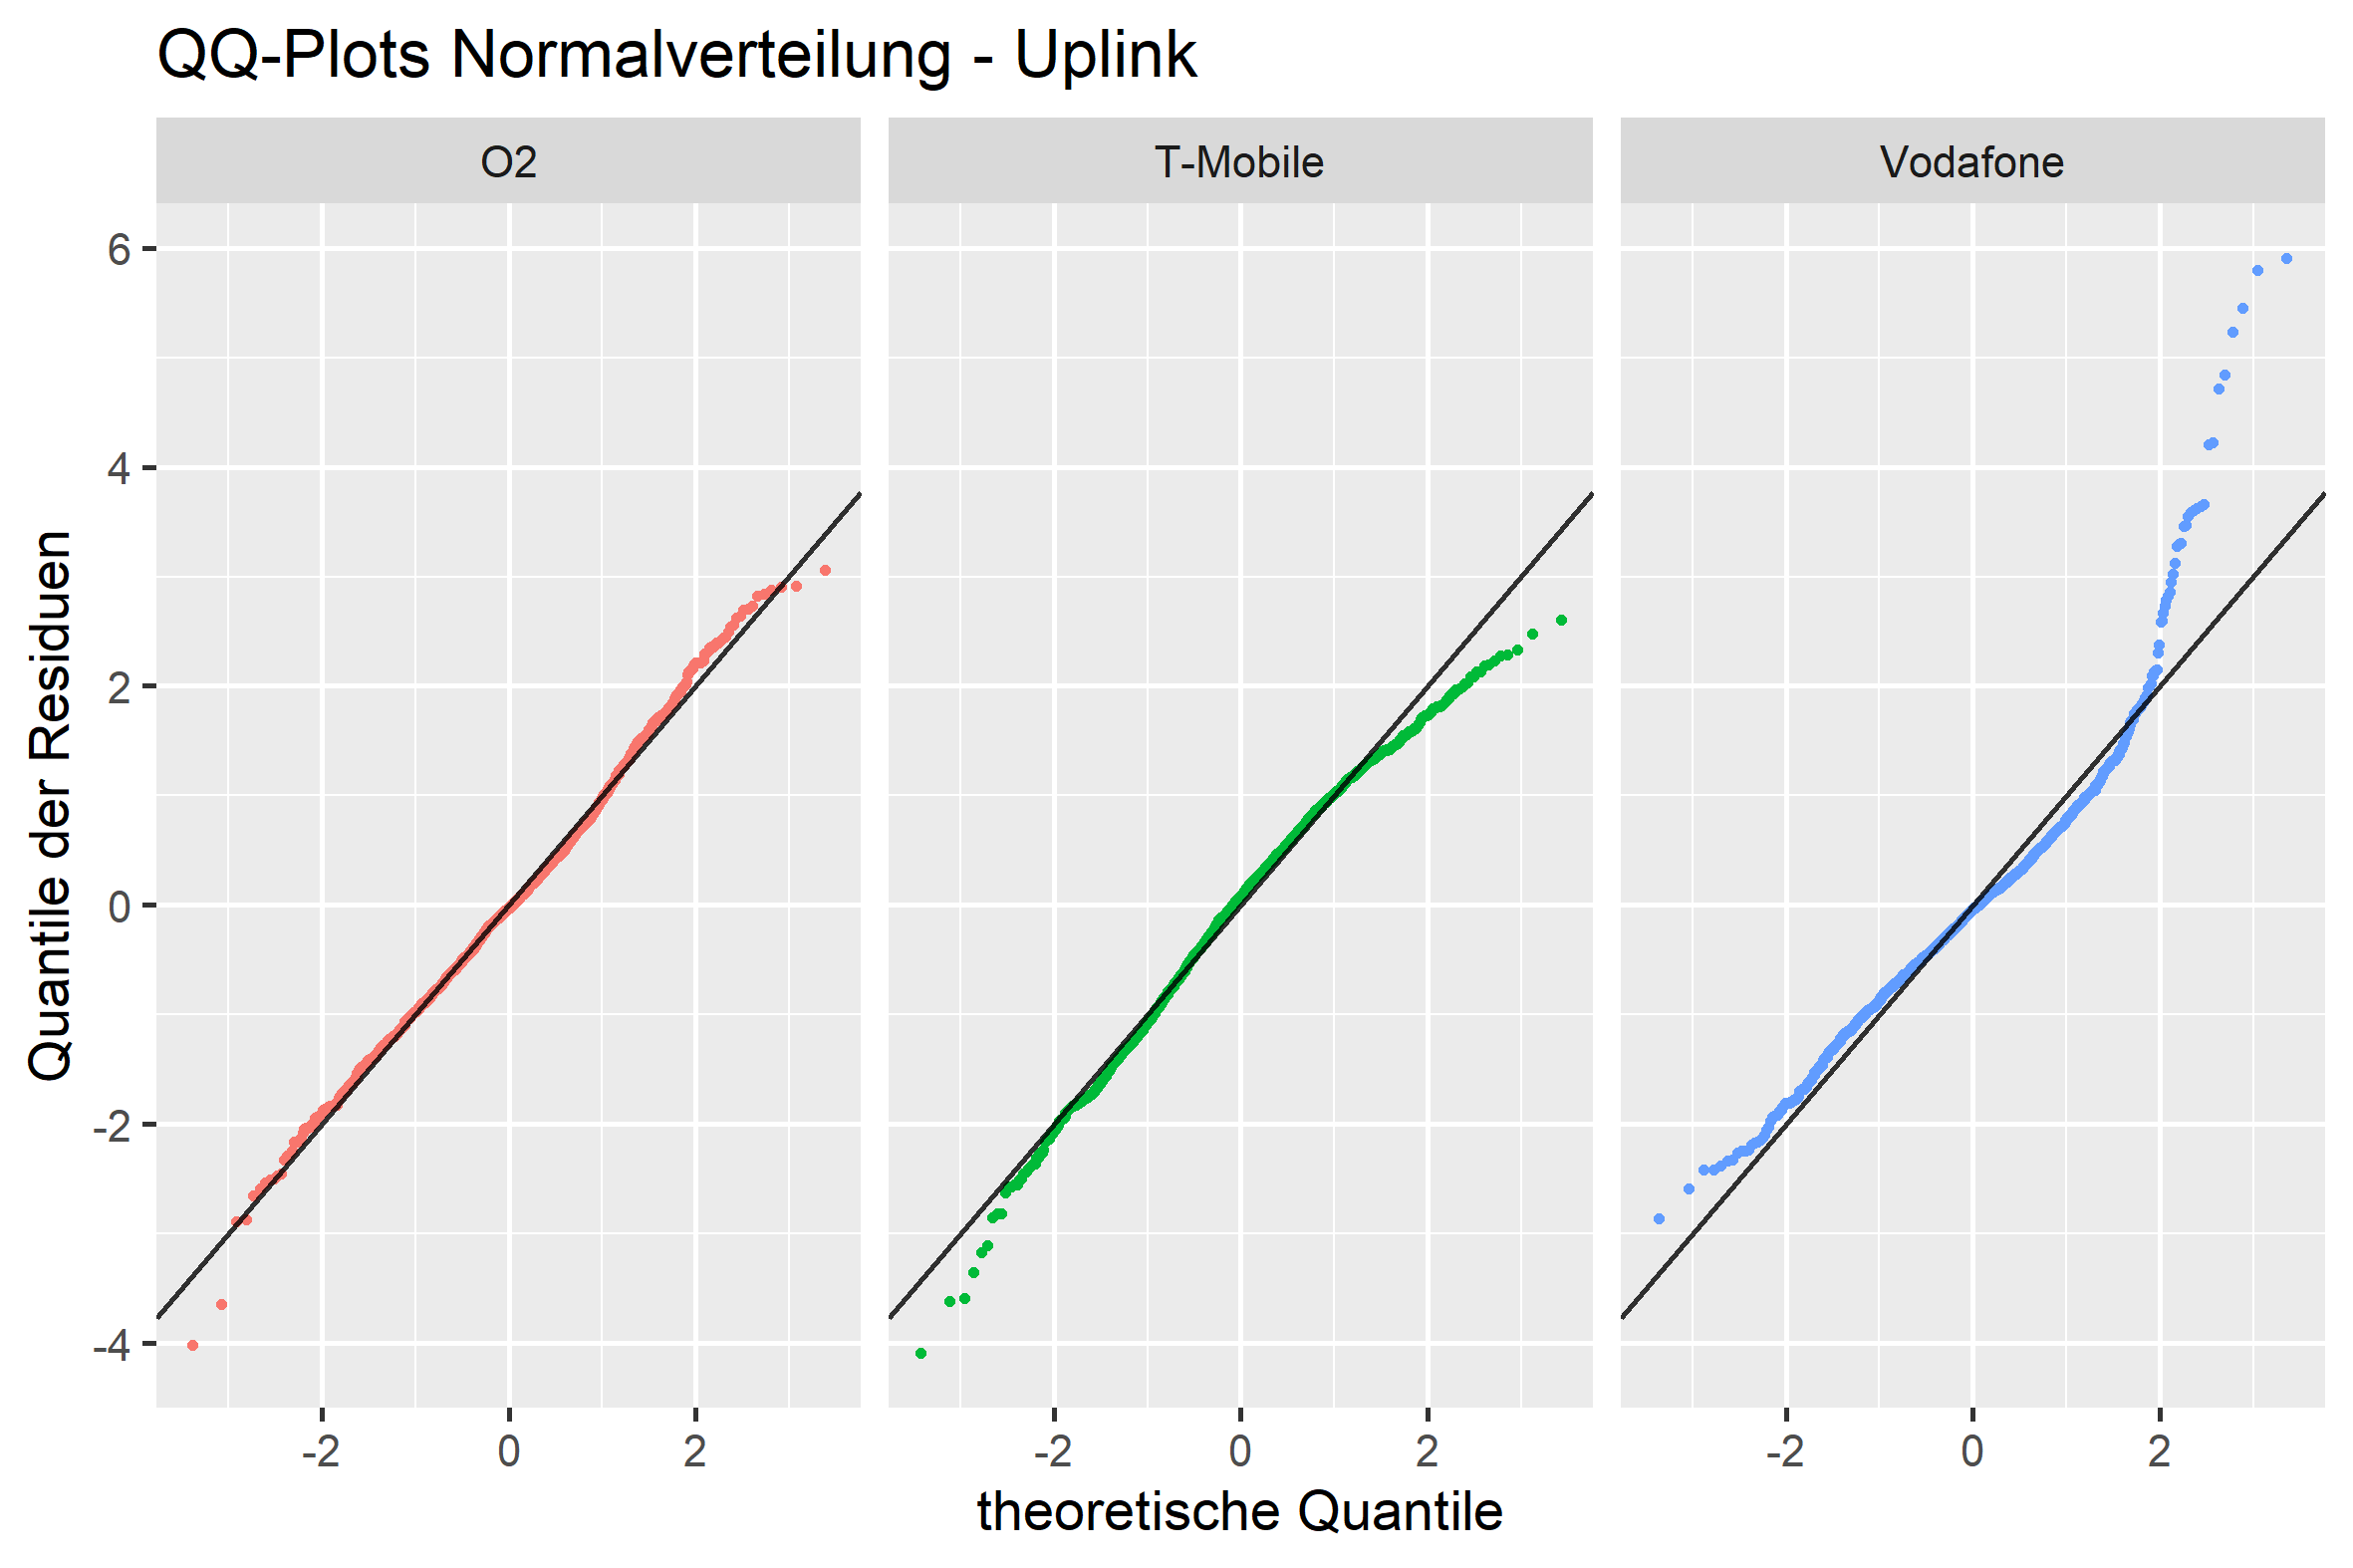
\includegraphics[scale=0.35]{plots/arima/uplink/res_qq}\\
		\caption{qq-Plots der Residuen der linearen Modelle mit Daten der Richtung Uplink.}
		\label{res_qq}
	\end{figure}
\end{frame}

\begin{frame}{Regression mit ARMA-Fehlern}
	\textbf{Bestimmung des Grids für die AR-Ordnung - Downlink}
	\begin{figure}
		%\centering
		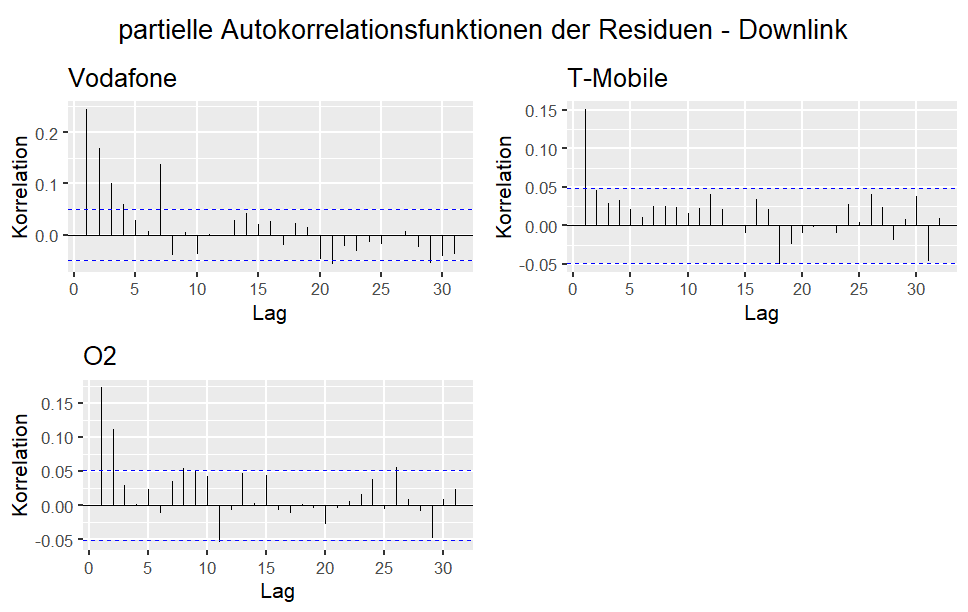
\includegraphics[scale=0.38]{plots/arima/downlink/res_pacf}\\
		\caption{Autokorrelationsfunktion der Residuen des linearen Modells in Richtung Downlink.}
		\label{res_pacf_dl}
	\end{figure}	
\end{frame}

\begin{frame}{Regression mit ARMA-Fehlern}
	\textbf{Bestimmung des Grids für die MA-Ordnung - Downlink}
	\begin{figure}
		%\centering
		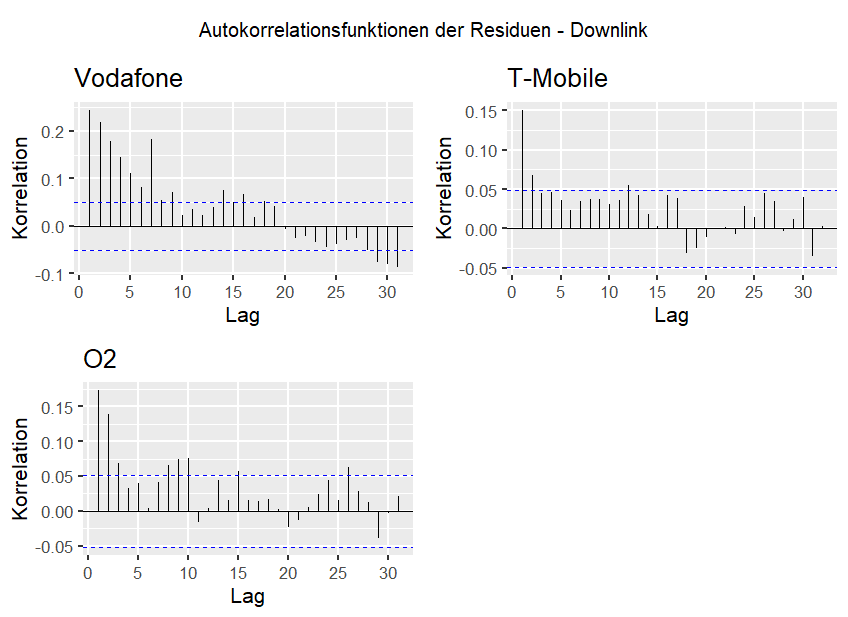
\includegraphics[scale=0.38]{plots/arima/downlink/res_acf}\\
		\caption{Autokorrelationsfunktion der Residuen des linearen Modells in Richtung Downlink.}
		\label{res_acf_dl}
	\end{figure}	
\end{frame}